% !TeX spellcheck = pt_BR

%%%%%%%%%%%%%%%%%%%%%%%%%%%%%%%%%%%%%%%%%%%%%%%
% Modelo adaptado do template original de
% Ted Pavlic (http://www.tedpavlic.com)
% Todos os créditos a ele.
%
% Na versão atual, o que foi modificado
% do original:
% Ajusta a numeração das questões e
% passa para português.
% Além de separar as configurações
% em um arquivo .cls separado.
%
% Crédito ao Roberto por ter feito
% a maior parte do trabalho de passar
% para o português e fazer outros
% ajustes para a versão atual deste template.
%%%%%%%%%%%%%%%%%%%%%%%%%%%%%%%%%%%%%%%%%%%%%%%


%----------------------------------------------------------------------------------------
%	PACKAGES E OUTRAS CONFIGURAÇÕES
%----------------------------------------------------------------------------------------

\documentclass{homeworkclass}

\usepackage{animate}


\usepackage{myMacros}


\hmwkTitle{Lista\ de\ Exercícios \#3}
\hmwkDueDate{Sábado,\ 27\ de\ Julho,\ 2019}
\hmwkClass{Elementos de Processamento de 	Sinais}
\hmwkClassTime{Segundas e Quartas (e Sextas): 08:00--10:00}
\hmwkClassInstructor{Prof.\ Sergio Lima Netto}
\hmwkAuthorName{Vinicius Mesquita de Pinho}
\hmwkAuthorShortName{Vinicius Mesquita}

\begin{document}

\maketitle

%----------------------------------------------------------------------------------------
%	SUMÁRIO
%----------------------------------------------------------------------------------------

%\setcounter{tocdepth}{1} % Uncomment this line if you don't want subsections listed in the ToC

\clearpage
\newpage
%\tableofcontents
%\newpage

%----------------------------------------------------------------------------------------
%	QUESTÃO 1
%----------------------------------------------------------------------------------------

% To have just one problem per page, simply put a \clearpage after each problem



\begin{homeworkProblem}[Filtros FIR usando o método de janelas.]	
Ao lançar mão das equações do livro-texto, pudemos desenvolver os filtros passa-bandas feitos com as seguintes janelas: retangular, Hamming, Hann, Blackman e Kaiser. Vamos observar as respostas em magnitude dos filtros, onde foi escolhida a banda de passagem entre $\pi/2 - 0.4$ e $\pi/2 + 0.4$, considerando o nosso espectro mostrado entre $0$ e $\pi$. Inicialmente, utilizaremos uma ordem $M = 50$. \\ A ordem pode parecer baixa, mas acho uma ordem dessa magnitude possibilita uma comparação visual entre as diferentes janelas. Vejamos por exemplo as respostas em magnitude de um filtro de janela retangular de ordem $M = 1000$ e outro feito com a janela de Hamming, com a mesma ordem. Ambos presentes na Figura~\ref{fig:milzera}.

\begin{figure}[!h]
	\centering
	\subfloat[Filtro de janela retangular.]{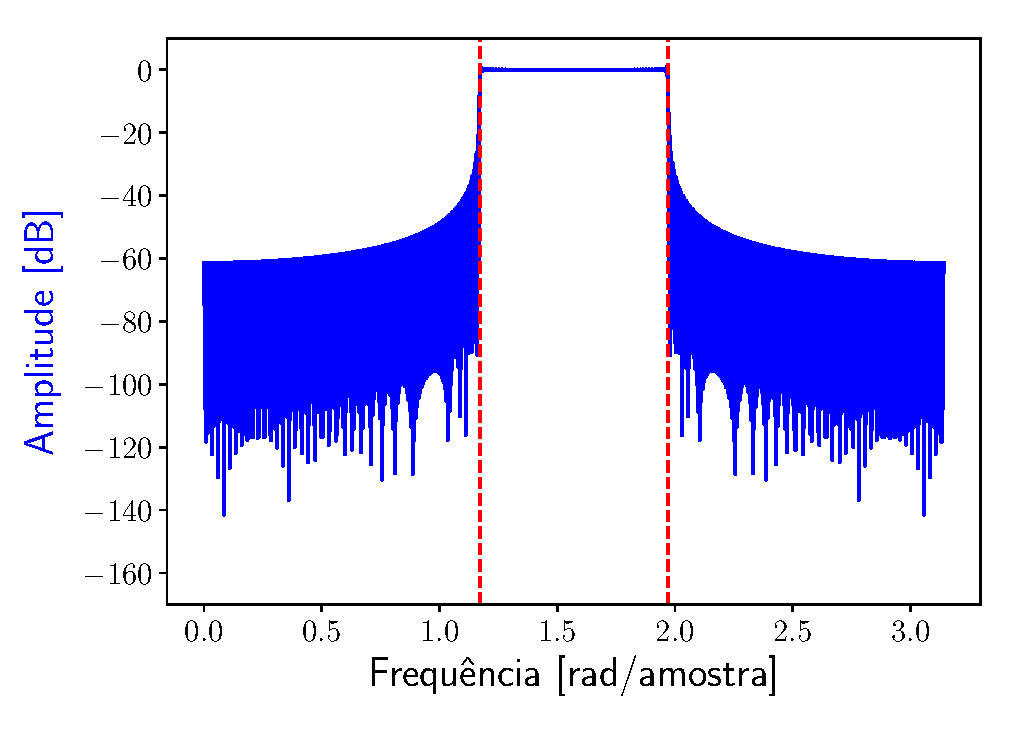
\includegraphics[width=0.45\linewidth]{figs/rect_milao}\label{fig:rect_milao}}
	~
	\subfloat[Filtro de janela de Hamming.]{\includegraphics[width=0.45\linewidth]{figs/hamming_milao}	\label{fig:hamming_milao}}
	
	\caption{Resposta em magnitude com ordem $M = 1000$.}
	\label{fig:milzera}
\end{figure}

Por mais que a janela de Hamming atenue mais fora da banda de passagem, uma ordem menor nos possibilita ver mais detalhes ainda, como veremos nos próximos exemplos. Vamos voltar para as ordens maiores depois.

Vou seguir a seguinte ordem, primeiro os filtros usando janela retangular, Hamming, Hann e Blackman. Depois vamos ver a janela de Kaiser e a influência do valor $\beta$. \\

Podemos ver nas Figuras~\ref{fig:rect_hamming_m_50}~e~\ref{fig:hann_blackman_50} as respostas em magnitude dos filtros. Com a mesma escala para todos, podemos ver que a janela de Blackman consegue a maior atenuação fora da banda passante, enquanto a janela retangular, a menor.
\begin{figure}[!h]
\centering
\subfloat[Janela retangular.]{\includegraphics[width=0.5\linewidth]{figs/rect}\label{fig:rect_50}}
~
\subfloat[Janela de Hamming.]{\includegraphics[width=0.5\linewidth]{figs/hamming}	\label{fig:hamming_50}}
\caption{Respostas em magnitude com ordem $M = 50$.}
\label{fig:rect_hamming_m_50}
\end{figure}

\pagebreak


\begin{figure}[!ht]
\subfloat[Janela de Hann.]{\includegraphics[width=0.5\linewidth]{figs/hann}	\label{fig:hann_50}}
~
\subfloat[Janela de Blackman]{\includegraphics[width=0.5\linewidth]{figs/blackman}	\label{fig:blackman_50}}

\caption{Respostas em magnitude com ordem $M = 50$.}
\label{fig:hann_blackman_50}
\end{figure}

Mas agora se traçarmos as linhas vermelhas que vemos na Figura~\ref{fig:hann_blackman_50_linha}, podemos ver que a janela retangular é que tem o menor ``vazamento'' para fora da faixa de frequências de interesse. Isso serve para vermos que não existe uma janela ideal e nem uma janela totalmente desprezível.

\begin{figure}[!h]
	\centering
	\subfloat[Janela retangular.]{\includegraphics[width=0.46\linewidth]{figs/rect_linha}\label{fig:rect_50_linha}}
	~
	\subfloat[Janela de Hamming.]{\includegraphics[width=0.46\linewidth]{figs/hamming_linha}	\label{fig:hamming_50_linha}}
	\\
	\subfloat[Janela de Hann.]{\includegraphics[width=0.46\linewidth]{figs/hann_linha}	\label{fig:hann_50_linha}}
	~
	\subfloat[Janela de Blackman]{\includegraphics[width=0.46\linewidth]{figs/blackman_linha}	\label{fig:blackman_50_linha}}
	
	\caption{Respostas em magnitude com ordem $M = 50$.}
	\label{fig:hann_blackman_50_linha}
\end{figure}

Mas, o jogo muda um pouco se pudermos ter uma ordem alta, como por exemplo $M = 1000$, a Figura~\ref{fig:hann_blackman_50_linha_milao} mostra as diferentes janelas para esse valor de $M$. Aqui podemos ver que a o ``vazamento'' para fora da faixa de interesse não é uma preocupação tão grande como anteriormente. Então poderíamos escolher uma janela de Blackman simplesmente por ela atenuar mais fora da faixa de interesse (isso porque não estamos levando em consideração complexidade de calcularmos o filtro e do filtro em si, etc.).

\begin{figure}[!h]
	\centering
	\subfloat[Janela retangular.]{\includegraphics[width=0.5\linewidth]{figs/rect_linha_milao}\label{fig:rect_50_linha_milao}}
	~
	\subfloat[Janela de Hamming.]{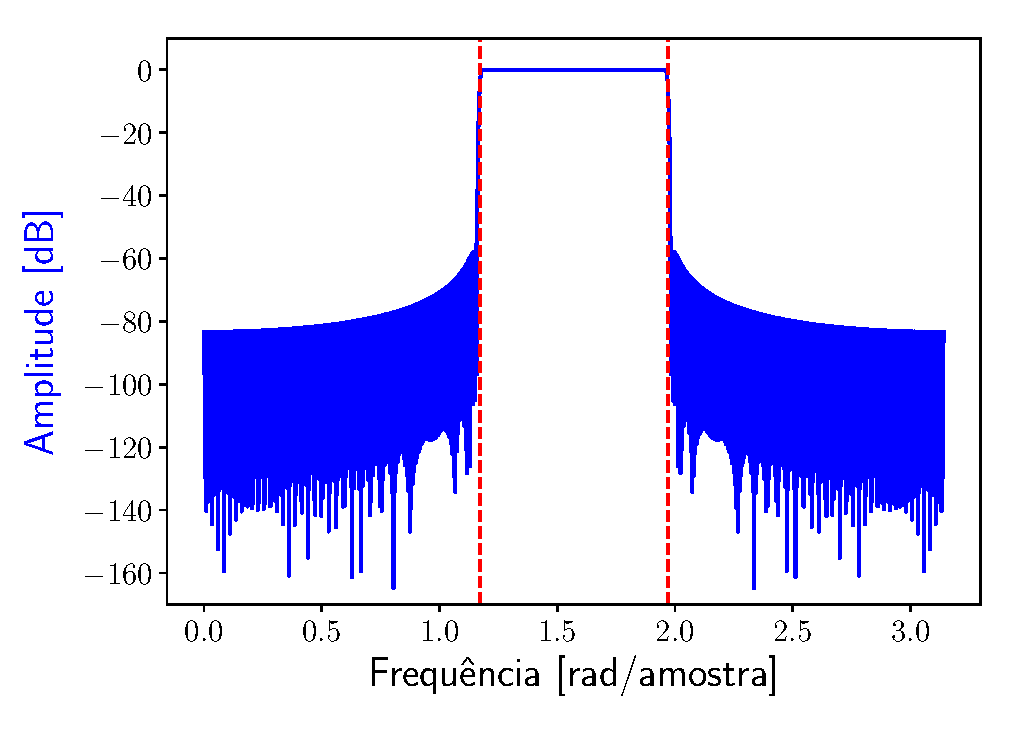
\includegraphics[width=0.5\linewidth]{figs/hamming_linha_milao}	\label{fig:hamming_50_linha_milao}}
	\\
	\subfloat[Janela de Hann.]{\includegraphics[width=0.5\linewidth]{figs/hann_linha_milao}	\label{fig:hann_50_linha_milao}}
	~
	\subfloat[Janela de Blackman]{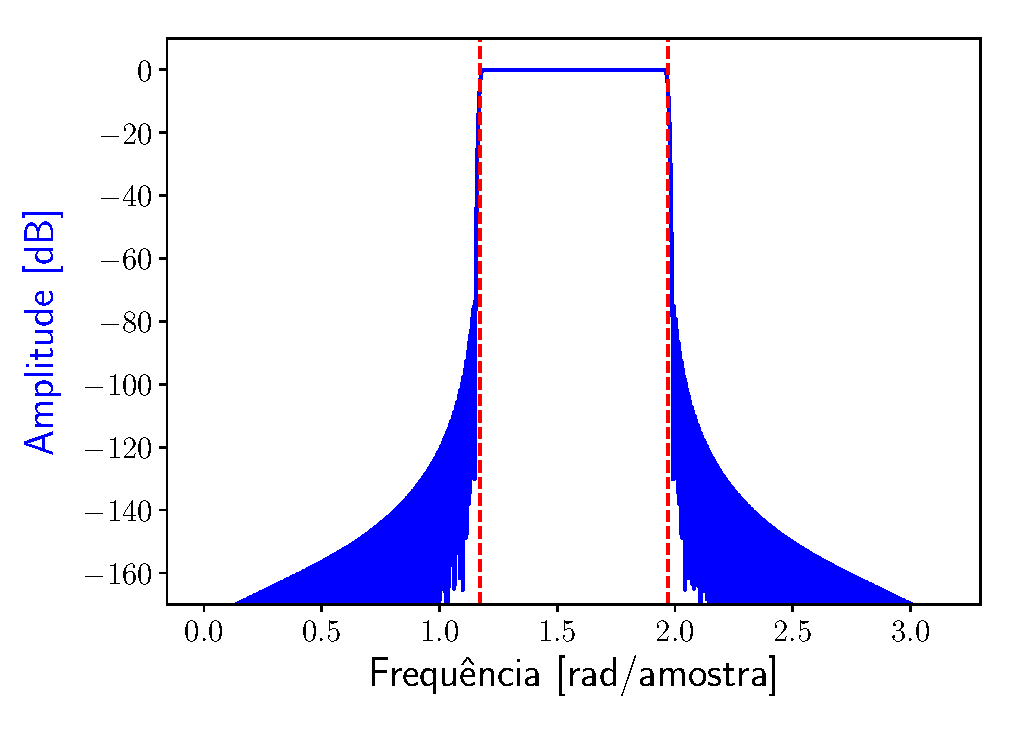
\includegraphics[width=0.5\linewidth]{figs/blackman_linha_milao}	\label{fig:blackman_50_linha_milao}}
	
	\caption{Respostas em magnitude com ordem $M = 1000$.}
	\label{fig:hann_blackman_50_linha_milao}
\end{figure}

Agora vamos observar a janela de Kaiser. Eu a deixei por último porque ela depende de uma parâmetro a mais que as outras. Enquanto as apresentadas até aqui dependeram apenas da ordem do filtro, a janela de Kaiser depende do valor $\beta$. O valor de $\beta$ é determinante para a relação entre a largura do lóbulo central e a amplitude do lóbulo lateral da janela (no tempo). Ao aumentarmos o $\beta$, a largura do lóbulo central diminui. Para alguns valores de $\beta$ a janela de Kaiser tem similaridades com as outras janelas observadas até aqui, para $\beta = 0$, temos uma janela próxima retangular, para $\beta = 5$, Hamming, $\beta = 6$, Hann, $\beta = 8.6$, Blackman. \\


Vamos observar o comportamento da janela com aumento de $\beta$. Na Figura~\ref{fig:kaiser_igual_as_outras}, podemos ver as similaridades com as janelas da Figura~\ref{fig:hann_blackman_50_linha} e como o ``vazamento'' para fora da faixa de interesse aumenta.

\begin{figure}[!h]
	\centering
	\subfloat[Janela Kaiser, $\beta = 0$.]{\includegraphics[width=0.5\linewidth]{figs/kaiser_0}\label{fig:kaiser_0}}
	~
	\subfloat[Janela Kaiser, $\beta = 5$.]{\includegraphics[width=0.5\linewidth]{figs/kaiser_5}	\label{fig:kaiser_5}}
	\\
	\subfloat[Janela Kaiser, $\beta = 6$.]{\includegraphics[width=0.5\linewidth]{figs/kaiser_6}	\label{fig:kaiser_6}}
	~
	\subfloat[Janela Kaiser, $\beta = 8.6$.]{\includegraphics[width=0.5\linewidth]{figs/kaiser_8_6}	\label{fig:kaiser_8_6}}
	
	\caption{Respostas em magnitude com ordem $M = 50$.}
	\label{fig:kaiser_igual_as_outras}
\end{figure}
\pagebreak
\vspace*{-1cm}
Para valores de $\beta = 10$ e $\beta = 15$, apresentados na Figura~\ref{fig:kaiser_beta_grande}, é preciso uma ordem bem maior para a especificação desejada.

\begin{figure}[!h]
	\centering
	\subfloat[Janela Kaiser, $\beta = 15$.]{\includegraphics[width=0.5\linewidth]{figs/kaiser_15}\label{fig:kaiser_15}}
	~
	\subfloat[Janela Kaiser, $\beta = 20$.]{\includegraphics[width=0.5\linewidth]{figs/kaiser_20}	\label{fig:kaiser_20}}

	
	\caption{Respostas em magnitude com ordem $M = 50$.}
	\label{fig:kaiser_beta_grande}
\end{figure}


\end{homeworkProblem}

\end{document}